% Provenance (never printed): see sources/outline_sources.md (Year 3:
% geophysical fluid dynamics: rotating-frame equations, Rossby number,
% hydrostatic and geostrophic balance, thermal wind, buoyancy frequency).
% Brief: sources/book5/BRIEFS.md, ch. 19. Curves from
% figdata/bachelor-3/inertial_oscillation.py, thermal_wind.py and
% buoyancy_frequency.py. Exercise and problem values in the Book 5 scratch
% calculator calc/ch19.py. The Steppe of Orrin, its lake, its stations and
% its winds are invented.
\chapter{ديناميكا الموائع الجيوفيزيائية}\label{ch:b3:gfd-foundations}

حرّك كوبًا من الشاي فيتلاشى الدوران خلال دقيقة، وتتجمّع أوراق الشاي
في وسط القاع، ولا يحدث شيء آخر. أمّا المحيط والغلاف الجوي
فيُحرَّكان أيضًا بفعل الشمس والرياح، لكن على كوكب دوّار وفي
طبقات مختلفة الكثافة. يجعلهما الدوران والتطبّق يخضعان
لقواعد لا يُظهرها فنجان الشاي: تهبّ الرياح موازيةً لخطوط تساوي الضغط لا عابرةً لها،
ولا تقبل أعمدة المائع أن تميل، وريح الطبقة العليا
من التروبوسفير تتحدّد بدرجات الحرارة الواقعة تحتها. يُرسي هذا الفصل
معادلات هذه التدفّقات الكبيرة البطيئة الرقيقة، والأعداد القليلة
التي تقرّر أيّ الحدود يُعتدّ بها.

\begin{recall}
قوى كوريوليس والطرد المركزي في إطار دوّار، ومعادلتا نافييه--ستوكس
والاستمرارية، واللزوجة، وعدد رينولدز، والعلاقة
الهيدروستاتيكية موجودة في كتب الفيزياء. ومعامل كوريوليس $f = 2\Omega
\sin\varphi$، وقوة تدرّج الضغط، والتوازن الجيوستروفي،
والرياح الجيوستروفية والتدرّجية والتيارات النفّاثة موجودة في مجلد
السنة الأولى، في فصله عن الدوران العام للغلاف الجوي؛ وطبقة إيكمان
في فصله عن دوران المحيط؛ ودرجة الحرارة الكامنة
والاستقرار السكوني واهتزاز كتلة هوائية مرفوعة في فصله عن بنية
الغلاف الجوي والمحيط.
\end{recall}

\section{المعادلات في إطار دوّار}\label{sec:b3:gfd-foundations:equations}

في إطار يدور مع الأرض بالسرعة الزاوية
$\vec\Omega$، تخضع كتلة مائع سرعتها $\vec u$ للمعادلتين الآتيتين
\[
\frac{\mathrm D\vec u}{\mathrm Dt} + 2\vec\Omega\times\vec u =
-\frac{1}{\rho}\nabla p + \vec g + \nu\nabla^2\vec u ,
\qquad
\frac{\partial\rho}{\partial t} + \nabla\cdot(\rho\vec u) = 0 ,
\]
حيث $\mathrm D/\mathrm Dt = \partial/\partial t + \vec u\cdot\nabla$ هي
المشتقة المتبعة للكتلة، و$\nu$ هي اللزوجة الحركية. وأُضيفت قوة الطرد المركزي إلى
الجاذبية: مجموعهما $\vec g$ هو الجاذبية الفعّالة، وهي
العمودية على السطوح المتساوية للجهد الأرضي،
ويُحدَّد الاتجاه الرأسي بها. لا يبقى من الدوران سوى حدّ كوريوليس $-2\vec\Omega\times
\vec u$، وهو لا يبذل شغلًا، إذ يُدير الكتلة
دون أن يغيّر سرعتها. وتدور الأرض بمعدّل $\Omega =
\qty{7.292115e-5}{rad/s}$، أي دورة واحدة كلّ يوم نجمي مدّته \qty{23.9345}{h}.
% ledger: geod5:grs80-defining, earth:Trot

بالنسبة إلى الحركة على مسافات أصغر بكثير من نصف قطر الأرض $a$، يكفي
إطار ديكارتي موضعي: $x$ شرقًا، و$y$ شمالًا، و$z$ نحو الأعلى،
عند خط العرض $\varphi$، أي المستوي المماسّ للشكل أدناه. وهنا
$\vec\Omega = \Omega\,(0, \cos\varphi, \sin\varphi)$، وتكون المركّبات الثلاث
لمعادلة كمية الحركة هي
\[
\begin{aligned}
\frac{\mathrm Du}{\mathrm Dt} - f v + \tilde f w &= -\frac{1}{\rho}\frac{\partial p}{\partial x} + F_x ,\\
\frac{\mathrm Dv}{\mathrm Dt} + f u &= -\frac{1}{\rho}\frac{\partial p}{\partial y} + F_y ,\\
\frac{\mathrm Dw}{\mathrm Dt} - \tilde f u &= -\frac{1}{\rho}\frac{\partial p}{\partial z} - g + F_z ,
\end{aligned}
\qquad f = 2\Omega\sin\varphi,\quad \tilde f = 2\Omega\cos\varphi ,
\]
حيث $\vec F$ قوة الاحتكاك. وبالنسبة إلى التدفّقات الرقيقة شبه الأفقية في
المحيط والغلاف الجوي تُهمَل الحدود المتضمّنة $\tilde f$: فالحدّ $\tilde f w$
صغير مقارنةً بالحدّ $fv$ لأنّ $w \ll v$، و$\tilde f u$ جزء من عشرة آلاف من
$g$ (انظر \cref{exo:b3:gfd-foundations:5}). وتؤثّر قوة كوريوليس عندئذٍ فقط في الاتجاه الأفقي،
عبر المركّبة الرأسية المحلية للدوران، أي
$\Omega\sin\varphi$.

\begin{definition}[المستوي $f$ والمستوي $\beta$]\label{def:b3:gfd-foundations:planes}
بالقرب من خط عرض مرجعي $\varphi_0$، يأخذ تقريب \emph{المستوي $f$}\index{المستوي $f$}
معامل كوريوليس ثابتًا، $f = f_0 =
2\Omega\sin\varphi_0$. أمّا تقريب \emph{المستوي $\beta$}\index{المستوي $\beta$}
يحتفظ بتغيّره من الرتبة الأولى مع المسافة نحو الشمال $y$:
$f = f_0 + \beta y$، حيث $\beta = \mathrm df/\mathrm dy = 2\Omega
\cos\varphi_0/a$.
\end{definition}

عند \ang{45}، ونصف القطر المتوسط $a = \qty{6371}{km}$، تكون $f_0 =
\qty{1.031e-4}{s^{-1}}$ و$\beta = \qty{1.62e-11}{m^{-1}.s^{-1}}$: على مسافة
\qty{1000}{km} من خط العرض يتغيّر $f$ بمقدار \qty{16}{\percent}. ويصلح المستوي $f$
للحركات الأصغر بكثير من ذلك، بينما يلزم المستوي $\beta$
من أجل التيارات الواسعة النطاق في الأحواض والموجات الكوكبية.
% ledger: earth:Rmean, geod5:grs80-defining (values in figdata/bachelor-3/inertial_oscillation.py)

\begin{omfigure}
\begin{minipage}[c]{0.42\linewidth}\centering
\begin{tikzpicture}[>=stealth, font=\small]
\draw[thick] (0,0) circle (2);
\draw[black!40, dashed] (-2,0) -- (2,0);
\draw[->, thick] (0,-2.4) -- (0,2.75) node[above] {$\vec\Omega$};
\draw (0,0) -- (30:2) coordinate (P);
\draw (0.6,0) arc (0:30:0.6);
\node at (15:0.9) {$\varphi$};
\draw[black!60] ($(P)+(120:-1.1)$) -- ($(P)+(120:1.3)$);
\draw[->, omThm, thick] (P) -- ++(0,1.6) node[right] {$\vec\Omega$};
\draw[->, omDef, thick] (P) -- ++(30:0.8) node[anchor=south west, align=left, inner sep=1pt] {\foreignlanguage{arabic}{\mbox{\textdir TLT $\Omega\sin\varphi$}،}\\\foreignlanguage{arabic}{نحو الأعلى}};
\draw[->, omMeth, thick] (P) -- ++(120:1.386) node[anchor=south, align=center, inner sep=1pt] {\foreignlanguage{arabic}{\mbox{\textdir TLT $\Omega\cos\varphi$}،}\\\foreignlanguage{arabic}{نحو الشمال}};
\draw[black!50, densely dotted] ($(P)+(30:0.8)$) -- ($(P)+(0,1.6)$) -- ($(P)+(120:1.386)$);
\draw (P) circle (0.09); \draw ($(P)+(-0.064,-0.064)$) -- ($(P)+(0.064,0.064)$);
\draw ($(P)+(-0.064,0.064)$) -- ($(P)+(0.064,-0.064)$);
\node[font=\scriptsize, anchor=west] at ($(P)+(0.14,-0.03)$) {\foreignlanguage{arabic}{\mbox{\textdir TLT $x$}، شرقًا}};
\node[font=\scriptsize, black!60] at (-1.15,-0.25) {خط الاستواء};
\end{tikzpicture}
\end{minipage}\hfill
\begin{minipage}[c]{0.55\linewidth}\centering
\begin{tikzpicture}
\begin{axis}[width=\linewidth, height=0.72\linewidth, xmin=0, xmax=90, ymin=0, ymax=1.8,
  xlabel={خط العرض \babelsublr{(\unit{\degree})}}, ylabel={معامل كوريوليس $f$ \babelsublr{($10^{-4}$\,\unit{s^{-1}})}},
  xtick={0,15,30,45,60,75,90}, tick label style={font=\scriptsize}, label style={font=\small},
  legend style={font=\scriptsize, draw=none, fill=none}, legend pos=north west]
% computed in figdata/bachelor-3/inertial_oscillation.py
\addplot[omDef, thick] table[x=lat, y=f] {figdata/out/bachelor-3-inertial_oscillation-fbeta.dat};
\addplot[omThm, densely dashed] table[x=lat, y=fb] {figdata/out/bachelor-3-inertial_oscillation-fbeta.dat};
\addplot[only marks, mark=*, mark size=1.6pt] coordinates {(45,1.03126)};
\legend{{$2\Omega\sin\varphi$}, {\foreignlanguage{arabic}{المستوي $\beta$ عند \mbox{\textdir TLT \ang{45}}}}}
\end{axis}
\end{tikzpicture}
\end{minipage}

\par\smallskip{\small يمينًا، الإطار المحلي عند خط العرض $\varphi$: $z$
على امتداد الرأسي المحلي، و$y$ شمالًا في المستوي المماسّ، و$x$ شرقًا
يتفرّع متجه الدوران إلى $\Omega\sin\varphi$ حول الرأسي،
الذي يُحوّل الحركة الأفقية، و$\Omega\cos\varphi$ حول المحور
الشمالي، ويُهمل في التدفّقات الرقيقة. يسارًا، معامل كوريوليس، ومستوي $\beta$
المماسّ له عند \ang{45}: قريب على نطاق من خطوط العرض، بعيد
عنه قرب خط الاستواء وقرب القطب.}\label{fig:b3:gfd-foundations:frame}
\end{omfigure}
% ledger: geod5:grs80-defining, earth:Rmean

تُبسّط تقريبان آخران المعادلات دون أن نفقد ما
يهمّ. ويتعلّق الأول بالكثافة.

\begin{definition}[تقريب بوسينسك]\label{def:b3:gfd-foundations:boussinesq}
يكتب \emph{تقريب بوسينسك}\index{تقريب بوسينسك} الكثافة
على الصورة $\rho = \rho_0 + \rho'$، حيث $\rho_0$ ثابت
و$|\rho'| \ll \rho_0$، ويُبقي على $\rho'$ فقط حيث تُضرب في $g$.
تصبح معادلة الاستمرار $\nabla\cdot\vec u = 0$، وتأخذ معادلة
كمية الحركة الشكلَ التالي:
\[
\frac{\mathrm D\vec u}{\mathrm Dt} + f\,\vec k\times\vec u =
-\frac{1}{\rho_0}\nabla p' + b\,\vec k + \nu\nabla^2\vec u ,
\qquad b = -g\,\frac{\rho'}{\rho_0} ,
\]
حيث $p'$ هو انحراف الضغط عن الضغط
الهيدروستاتيكي للكثافة $\rho_0$، و$\vec k$ متجهُ الوحدة نحو الأعلى، و$b$
الطفو.
\end{definition}

في المحيط تكون $\rho'$ بضعة \unit{kg/m^3} على \num{1025}، أي كسرًا من
المائة، والتقريب ممتاز. وفي الغلاف الجوي تنخفض الكثافة
بمقدار عامل $e$ في نحو \qty{8.5}{km}؛ ويصحّ التقريب للطبقات
الأرقّ بكثير من ذلك، وتستبدل التدفّقات الأعمق $\rho_0$ بتابع
متوسّط $\rho_0(z)$، مع بقاء الفيزياء نفسها.
% ledger: earth:Hscale

يكون المائع الساكن في توازن هيدروستاتيكي. ويحافظ المائع المتحرّك على هذا التوازن
بتقريب جيد جدًّا عندما تكون الحركة
أوسع بكثير من عمقها.

\begin{definition}[التقريب الهيدروستاتيكي]\label{def:b3:gfd-foundations:hydrostatic}
يستبدل \emph{التقريب الهيدروستاتيكي}\index{التقريب الهيدروستاتيكي}
معادلة كمية الحركة الرأسية لمائع متحرّك بالعلاقة
الهيدروستاتيكية، $\partial p/\partial z = -\rho g$.
\end{definition}

\begin{proposition}[متى يكون التقريب الهيدروستاتيكي صحيحًا]\label{prop:b3:gfd-foundations:hydrostatic}
بالنسبة إلى حركة ذات مقياس أفقي $L$ وعمق $H$ وسرعة $U$، مع \omterm{def:b3:gfd-foundations:numbers}{عدد
روسبي} $U/(fL)$ لا يتجاوز مرتبة الواحد، يكون التسارع الرأسي
أصغر من التدرّج الرأسي لاضطراب الضغط بعامل
من مرتبة $(U/fL)\,(H/L)^2$.
\end{proposition}

\begin{proof}
عندما تكون قوة كوريوليس على الأقلّ بقدر التسارع، توازن
معادلة كمية الحركة الأفقية تدرّجَ الضغط الأفقي مقابلها:
$p'/(\rho_0 L) \sim fU$، ومنه $p'/\rho_0 \sim fUL$، والتدرّج الرأسي
هو $p'/(\rho_0 H) \sim fUL/H$. تُعطي معادلة الاستمرار $\partial w/\partial z
= -(\partial u/\partial x + \partial v/\partial y)$، وتُقيّد السرعة الرأسية
بالقيمة $W \sim UH/L$، والتسارع الرأسي بالقيمة
$\mathrm Dw/\mathrm Dt \sim UW/L = U^2H/L^2$. والنسبة هي $(U^2H/L^2)/(fUL/H)
= (U/fL)(H/L)^2$.
\end{proof}

لمنظومة طقس عرضها \qty{1000}{km} في التروبوسفير عمقه \qty{10}{km}
تكون $(H/L)^2 = 10^{-4}$ \omterm{def:b3:gfd-foundations:numbers}{وعدد روسبي} نحو 0.1: يبلغ
خطأ \omterm{def:b3:gfd-foundations:hydrostatic}{التقريب الهيدروستاتيكي} من مرتبة $10^{-5}$. ولا يفشل إلا في الحركات الضيّقة العميقة:
تيّار صاعد من عاصفة رعدية، وعمود حملي في المحيط.

\section{مقاييس التدفّق الدوّار}\label{sec:b3:gfd-foundations:scales}

تتحدّد الحدود ذات الأهمية في معادلة كمية الحركة بنسبتين.

\begin{definition}[عددا روسبي وإيكمان]\label{def:b3:gfd-foundations:numbers}
بالنسبة إلى تدفّق سرعته $U$ ومقياسه الأفقي $L$ وعمقه $H$ على كوكب ذي
معامل كوريوليس $f$، يكون \emph{عدد روسبي}\index{عدد روسبي} هو
$\mathrm{Ro} = U/(fL)$، أي نسبة التسارع، من مرتبة $U^2/L$،
إلى قوة كوريوليس، من مرتبة $fU$. أمّا \emph{عدد إيكمان}\index{عدد إيكمان}
فهو $\mathrm{Ek} = \nu/(fH^2)$، أي نسبة
قوة اللزوجة، من مرتبة $\nu U/H^2$، إلى قوة كوريوليس؛ وفي
التدفّق المضطرب يُستبدل $\nu$ بلزوجة الاضطراب الدوّامي.
\end{definition}

لحوض استحمام يُفرَغ بسرعة \qty{0.1}{m/s} على مسافة \qty{0.3}{m} عددُ روسبي له
بضعة آلاف: لا يحدّد دوران الأرض اتجاه دوامته.
لمنخفض جوّي عرضه \qty{1000}{km} تهبّ فيه رياح بسرعة \qty{15}{m/s}،
يبلغ عددُ روسبي له $\mathrm{Ro} \approx 0.14$، وللدوّامة المحيطية $\mathrm{Ro} \sim 10^{-4}$.
اللزوجة أضعف من ذلك: تبلغ اللزوجة الجزيئية للماء
\qty{e-6}{m^2/s}، أمّا لزوجات الاضطراب الدوّامي التي تمثّل
اضطراب المحيط، \qtyrange{e-5}{e-3}{m^2/s} في الاتجاه الرأسي، فتعطي
$\mathrm{Ek} \sim 10^{-5}$ على عمق \qty{1000}{m}. ويرتبط العددان
بعدد رينولدز بالعلاقة $\mathrm{Re} = UL/\nu =
(\mathrm{Ro}/\mathrm{Ek})(L/H)^2$.
% ledger: stewart:eddy (problem values in calc/ch19.py)

عندما يكون العددان صغيرين، تُبقي معادلة كمية الحركة الأفقية المستقرّة
على قوة كوريوليس وتدرّج الضغط فقط: يكون التدفّق في
توازن جيوستروفي، $f\,\vec k\times\vec u_g = -(1/\rho)\nabla_h p$، وهو
ما قرأه مجلد السنة الأولى من خرائط الطقس. والجيوستروفية هي الحالة الحدّية
حين $\mathrm{Ro}, \mathrm{Ek}\to 0$؛ وتصحيحاتها من مرتبة
$\mathrm{Ro}$، ولا يؤثّر الاحتكاك إلا في طبقات ذات سُمك نسبي
$\sqrt{\mathrm{Ek}}$، وهي طبقات إيكمان عند قاع الغلاف الجوي
وأعلى المحيط وقاعه. وعلى المستوي $f$ تكون السرعة الجيوستروفية
خالية من التباعد الأفقي: $\partial u_g/\partial x + \partial
v_g/\partial y = -(1/\rho f)(\partial^2 p/\partial x\partial y -
\partial^2 p/\partial y\partial x) = 0$ إذا كانت $\rho$ منتظمة.

النهاية المعاكسة، أي الدوران بلا تدرّج للضغط، هي أبسط
حركة يمكن لمائع دوّار أن يقوم بها.

\begin{definition}[الاهتزاز القصوري]\label{def:b3:gfd-foundations:inertial}
\emph{الاهتزاز القصوري}\index{الاهتزاز القصوري} هو
الحركة الأفقية لمائع لا تؤثّر فيه أيّ قوّة أفقية
سوى قوّة كوريوليس.
\end{definition}

\begin{theorem}[الدوائر القصورية]\label{thm:b3:gfd-foundations:inertial}
على المستوي $f$، جسيمة مائع تتحرّك بسرعة $U$ دون أيّ قوّة أفقية
سوى قوّة كوريوليس تحتفظ بسرعتها وتصف دائرة نصف قطرها
$U/|f|$، في اتجاه عقارب الساعة في نصف الكرة الشمالي وعكسه في الجنوبي،
ودورها القصوري $2\pi/|f|$، وهو نصف يوم نجمي
مقسومًا على $\sin\varphi$.
\end{theorem}

\begin{proof}
المعادلتان هما $\mathrm du/\mathrm dt = fv$، $\mathrm dv/\mathrm dt =
-fu$. مع $w = u + \mathrm iv$ تصبحان $\mathrm dw/\mathrm dt = -\mathrm
if\,w$، إذن $w = U\,\mathrm e^{-\mathrm ift}$ في حال البدء شرقًا، فإنّ
السرعة $|w| = U$ ثابتة، ويدور متجه السرعة بالمعدّل $f$،
في اتجاه عقارب الساعة عندما $f > 0$. وبالتكامل، يدور الموضع $x + \mathrm iy =
(\mathrm iU/f)(\mathrm e^{-\mathrm ift} - 1)$ حول النقطة
$-\mathrm iU/f$ على بعد $U/|f|$. ودور الحركة هو $2\pi/|f| =
2\pi/(2\Omega|\sin\varphi|)$، و$2\pi/\Omega$ هو اليوم النجمي.
\end{proof}

عند \ang{45} يبلغ الدور القصوري \qty{16.9}{h}، ويدور تيّار مقداره
\qty{0.2}{m/s} على دائرة نصف قطرها \qty{1.94}{km}؛ وعند \ang{30} يكون الدور
يومًا نجميًا كاملًا، وعند خطّ الاستواء لا توجد دوائر قصورية.
بعد أن حرّكت عاصفة طبقة سطح المحيط ثمّ هدأت،
يفعل الماء هذا تمامًا. وعوامات الانجراف المزوّدة بمظلّة بحرية عند \qty{15}{m} في
شمال المحيط الهادئ رسمت حلقات لعدّة أيّام بعد عاصفة في أكتوبر 1987، محمولةً
بالتيّار المتوسّط: المسار الثالث في الشكل أدناه، بعد
الدائرة والحلزون.
% ledger: stewart:inertial, earth:Trot (values in figdata/bachelor-3/inertial_oscillation.py)

\begin{omfigure}
\begin{tikzpicture}
\begin{axis}[width=\linewidth, axis equal image, xmin=-3, xmax=18.5, ymin=-4.6, ymax=1.2,
  xlabel={المسافة نحو الشرق \babelsublr{(km)}}, ylabel={المسافة نحو الشمال \babelsublr{(km)}},
  tick label style={font=\scriptsize}, label style={font=\small},
  legend style={font=\scriptsize, draw=none, fill=white, fill opacity=0.85, text opacity=1},
  legend pos=south east, legend columns=3]
% computed in figdata/bachelor-3/inertial_oscillation.py
\addplot[black!45, line width=1.6pt] table[x=x, y=y] {figdata/out/bachelor-3-inertial_oscillation-circle.dat};
\addplot[omDef, thick] table[x=x, y=y] {figdata/out/bachelor-3-inertial_oscillation-spiral.dat};
\addplot[omThm, thick] table[x=x, y=y] {figdata/out/bachelor-3-inertial_oscillation-loops.dat};
\addplot[only marks, mark=*, mark size=1.8pt] coordinates {(0,0)};
\legend{{بلا احتكاك}, {احتكاك}, {احتكاك وتيّار}}
\end{axis}
\end{tikzpicture}

\par\smallskip{\small مسارات على مدى أربعة أيّام لجسيمة مائع تتحرّك
شرقًا بسرعة \qty{0.2}{m/s} عند \ang{45}~شمالًا (النقطة)، دون أيّ قوّة إلا قوّة
كوريوليس: دائرة نصف قطرها \qty{1.94}{km} تُقطع في اتجاه عقارب الساعة كلّ
\qty{16.9}{h} (رمادي)؛ ومع احتكاك يُنقص السرعة إلى النصف خلال
\num{2.8}~يومًا، حلزون متّجه نحو الداخل (أزرق)؛ والمسار نفسه محمولًا بتيّار ثابت
متّجه شرقًا بمقدار \qty{0.05}{m/s}، سلسلة من حلقات متناقصة الحجم
(أحمر).}\label{fig:b3:gfd-foundations:inertial}
\end{omfigure}
% ledger: stewart:inertial

يقع بين الجيوستروفية والدائرة القصورية الجريان حول مركز
ضغط مرتفع أو منخفض، حيث تكون خطوط تساوي الضغط منحنية، ولم يعد
التسارعُ باتّجاه المركز مهملًا.

\begin{definition}[الريح التدرّجية]\label{def:b3:gfd-foundations:gradient}
\emph{الريح التدرّجية}\index{الريح التدرّجية} هي الجريان الثابت عديم
الاحتكاك على طول خطوط تساوي الضغط المنحنية، تتوازن فيه قوّة تدرّج الضغط، وقوّة
كوريوليس، والتسارع المركزي.
\end{definition}

\begin{proposition}[تصحيح الانحناء]\label{prop:b3:gfd-foundations:gradient}
لتكن خطوط تساوي الضغط دوائر نصف قطرها $r$ في نصف الكرة الشمالي،
و$V_g$ السرعة الجيوستروفية التي يعطيها تدرّج ضغطها، مع
$\mathrm{Ro}_g = V_g/(fr)$. حول منخفض، تكون \omterm{def:b3:gfd-foundations:gradient}{الريح التدرّجية}
$V = 2V_g/(1 + \sqrt{1 + 4\mathrm{Ro}_g})$، أبطأ من $V_g$؛ وحول مرتفع،
$V = 2V_g/(1 + \sqrt{1 - 4\mathrm{Ro}_g})$، أسرع، ولا توجد إلا
إذا كان $\mathrm{Ro}_g \le 1/4$. وبالتقريب من الدرجة الأولى، $V = V_g(1 \mp \mathrm{Ro}_g)$.
\end{proposition}

\begin{proof}
حول المنخفض تدور الريح عكس اتجاه عقارب الساعة؛ وقوّة تدرّج الضغط
$fV_g$ تتّجه نحو المركز، وقوّة كوريوليس $fV$ نحو الخارج، والفرق بينهما
يوفّر التسارع المركزي: $fV_g - fV = V^2/r$. والجذر الموجب للمعادلة
$V^2 + frV - frV_g = 0$ هو $V = (fr/2)(\sqrt{1 +
4\mathrm{Ro}_g} - 1)$؛ وبضرب البسط والمقام في $(\sqrt{1 + 4\mathrm{Ro}_g} +
1)/(\sqrt{1 + 4\mathrm{Ro}_g} + 1)$ نحصل على الصيغة. وحول المرتفع،
تدور الريح في اتجاه عقارب الساعة وتتّجه قوّة كوريوليس نحو الداخل: $fV - fV_g =
V^2/r$، إذن $V^2 - frV + frV_g = 0$، وهذه لها جذور حقيقية فقط إذا كان $f^2r^2
\ge 4frV_g$؛ والجذر الذي يؤول إلى $V_g$ عندما $\mathrm{Ro}_g \to 0$ هو
$V = (fr/2)(1 - \sqrt{1 - 4\mathrm{Ro}_g})$. وبنشر الجذور التربيعية،
نجد $V = V_g(1 \mp \mathrm{Ro}_g + \dots)$.
\end{proof}

يقيس \omterm{def:b3:gfd-foundations:numbers}{عدد روسبي} لخطوط تساوي الضغط حجم التصحيح، وهو نحو عُشر في
حالة منخفض متوسّط الحجم. والشرط $\mathrm{Ro}_g \le 1/4$ هو سبب
لماذا يتّسم مركز المرتفع الجوي بتدرّجات ضعيفة ورياح خفيفة، بينما
أمّا مركز المنخفض فيمكن أن يحمل تدرّجات شديدة وعواصف.

\section{الدوران دون تطبّق}\label{sec:b3:gfd-foundations:taylor}

يسلك مائع دوّار ذو كثافة منتظمة، في حركة بطيئة، كما لو كان
مؤلَّفًا من أعمدة صلبة موازية لمحور الدوران.

\begin{theorem}[تايلور--برودمان]\label{thm:b3:gfd-foundations:taylor-proudman}
في جريان ثابت لمائع عديم اللزوجة منتظم الكثافة، يدور بالمتجه
$\vec\Omega$، ومع \omterm{def:b3:gfd-foundations:numbers}{عدد روسبي} صغير، لا تتغيّر متجهة السرعة على طول
اتّجاه محور الدوران: $(\vec\Omega\cdot\nabla)\vec u = 0$.
\end{theorem}
\index{مبرهنة تايلور--برودمان}

\begin{proof}
لمّا يؤول $\mathrm{Ro}\to 0$، ويكون الجريان ثابتًا عديم اللزوجة، تُختزل معادلة الزخم
إلى $2\vec\Omega\times\vec u = -\nabla(p/\rho_0 + \Phi)$، حيث $\Phi$ هو
\omterm{def:b3:gravity-geodesy:geopotential}{الجهد الأرضي}. وتنعدم دوّامة التدرّج، فيكون $\nabla\times(\vec\Omega
\times\vec u) = 0$. وبالنسبة إلى $\vec\Omega$ ثابتة، تساوي هذه الدوّامة $\vec\Omega
(\nabla\cdot\vec u) - (\vec\Omega\cdot\nabla)\vec u$، و$\nabla\cdot\vec u
= 0$ مع منتظمية الكثافة.
\end{proof}

مع كون $\vec\Omega$ موازية للمحور $z$، يكون $\partial\vec u/\partial z = 0$: تتساوى المركّبات الثلاث
للسرعة على كل ارتفاع. وإذا منعت قاعدة صلبة
$w$ عندها، فإنّ $w = 0$ في كل مكان، ويكون الجريان الأفقي واحدًا على كل مستوى.
ومن ثمّ يُحسّ عائق على قاع خزّان دوّار بتأثيره حتى
السطح: إذ لا يستطيع المائع الذي فوقه أن يتجاوزه صعودًا، لأنّ ذلك
يمطّ عمودًا أو يضغطه، فيلتفّ حوله على كل ارتفاع.
وعمود المائع الذي يبقى فوق العائق يُسمّى \emph{عمود
تايلور}\index{عمود تايلور}.

\begin{omfigure}
\begin{tikzpicture}[>=stealth, font=\small]
% side view
\fill[omDef!8] (0,0) rectangle (5.4,3);
\fill[black!10] (2.1,0) rectangle (3.3,3);
\draw[thick] (0,3.3) -- (0,0) -- (5.4,0) -- (5.4,3.3);
\draw[black!50] (0,3) -- (5.4,3);
\draw[fill=black!45] (2.1,0) .. controls (2.4,0.55) and (3.0,0.55) .. (3.3,0) -- cycle;
\draw[black!60, densely dashed] (2.1,0) -- (2.1,3) (3.3,0) -- (3.3,3);
\foreach \y in {0.8,1.6,2.4} {\draw[->, omDef, thick] (0.3,\y) -- (1.9,\y);
  \draw[->, omDef, thick] (3.5,\y) -- (5.1,\y);}
\draw[->, thick, omThm] (2.7,3.25) -- (2.7,4.0) node[right] {$\vec\Omega$};
\node[font=\scriptsize, align=center] at (2.7,1.7) {\foreignlanguage{arabic}{عمود}\\\foreignlanguage{arabic}{تايلور}};
\node[font=\scriptsize, anchor=north] at (2.7,-0.05) {{\foreignlanguage{arabic}{عائق}}};
\node[font=\small] at (2.7,-0.6) {{\foreignlanguage{arabic}{(أ) منظر جانبي}}};
% top view
\begin{scope}[xshift=6.4cm]
\fill[omDef!8] (0,0) rectangle (5.4,3);
\draw[thick] (0,0) rectangle (5.4,3);
\fill[black!10] (2.7,1.5) circle (0.5);
\draw[black!60, densely dashed] (2.7,1.5) circle (0.5);
\foreach \d/\h in {0.3/0.10, 0.75/0.35, 1.2/0.58} {
  \draw[->, omDef, thick] (0.2,1.5+\d) .. controls (1.6,1.5+\d) and (2.0,1.5+\h+0.62) .. (2.7,1.5+\h+0.62)
     .. controls (3.4,1.5+\h+0.62) and (3.8,1.5+\d) .. (5.2,1.5+\d);
  \draw[->, omDef, thick] (0.2,1.5-\d) .. controls (1.6,1.5-\d) and (2.0,1.5-\h-0.62) .. (2.7,1.5-\h-0.62)
     .. controls (3.4,1.5-\h-0.62) and (3.8,1.5-\d) .. (5.2,1.5-\d);}
\node[font=\small] at (2.7,-0.6) {{\foreignlanguage{arabic}{(ب) منظر من الأعلى، على أيّ ارتفاع}}};
\end{scope}
\end{tikzpicture}

\par\smallskip{\small \omterm{thm:b3:gfd-foundations:taylor-proudman}{عمود تايلور} (تخطيطي). (أ) في خزّان من الماء المنتظم
يدور بسرعة، يلتقي جريان بطيء بعائق منخفض على
القاع؛ يبقى المائع فوق العائق (الرمادي) محتجزًا حتى
السطح، ويلتفّ الجريان على كل ارتفاع حول العمود كأنّ
العائق يبلغ القمة. (ب) الجريان المرئي من الأعلى واحد عند
كل مستوى.}\label{fig:b3:gfd-foundations:taylor}
\end{omfigure}

الغلاف الجوي والمحيط متطبّقان، ويُخفّف التطبّق من القيد:
فالمائع المتطبّق يمكن أن يتغيّر مع الارتفاع، على النحو الذي
تفرضه مبرهنة \omterm{thm:b3:gfd-foundations:thermal-wind}{الريح الحرارية}.

\section{التطبّق والريح الحرارية}\label{sec:b3:gfd-foundations:stratification}

رفع مجلد السنة الأولى طردًا هوائيًّا في غلاف جوي مستقرّ، فوجد
أنّه يهتزّ حول مستواه. والأمر نفسه في أيّ مائع متطبّق،
وتردّد الاهتزاز هو مقياس التطبّق.

\begin{definition}[تردّد الطفو]\label{def:b3:gfd-foundations:buoyancy}
يُعرَّف \emph{تردّد الطفو}\index{تردّد الطفو} $N$ لمائع
ساكن بالعلاقة
\[
N^2 = \frac{g}{\theta}\frac{\mathrm d\theta}{\mathrm dz}\ \text{(الهواء)},
\qquad
N^2 = -\frac{g}{\rho_0}\frac{\mathrm d\rho_\theta}{\mathrm dz}\ \text{(ماء البحر)},
\]
حيث $\theta$ هي درجة الحرارة الكامنة للهواء، و$\rho_\theta$ الكثافة
الكامنة للماء، أي الكثافة التي يبلغها لو نُقل أديباتيًّا
إلى ضغط مرجعي.
\end{definition}

\begin{theorem}[اهتزاز طرد مزاح]\label{thm:b3:gfd-foundations:buoyancy}
يخضع طرد يُزاح رأسيًّا مسافة صغيرة $\zeta$ عن مستواه في
مائع ساكن، أديباتيًّا ودون امتزاج، للمعادلة $\ddot\zeta =
-N^2\zeta$. فإذا كان $N^2 > 0$ يهتزّ بالتردّد الزاوي $N$؛ وإذا
كان $N^2 < 0$ تكبر الإزاحة ويكون المائع غير مستقرّ.
\end{theorem}

\begin{proof}
يُحفظ الطرد المنقول أديباتيًّا ودون امتزاج كثافته الكامنة
$\rho_\theta(z_0)$. وعند المستوى $z_0 + \zeta$ يكون عند ضغط محيطه،
وكثافته الكامنة $\rho_\theta(z_0) +
\zeta\,\mathrm d\rho_\theta/\mathrm dz$؛ ويختلف طردان عند الضغط نفسه
في الكثافة بقدر فرق كثافتيهما الكامنتين، بالتقريب من
الرتبة الأولى. وقوة الطفو لكل وحدة كتلة هي $-g(\rho_p - \rho_e)/\rho_0 =
g\,\zeta\,(\mathrm d\rho_\theta/\mathrm dz)/\rho_0 = -N^2\zeta$. وبالنسبة إلى الهواء عند
ضغط معيّن تتغيّر الكثافة كالمقلوب $1/\theta$، فيكون $-\mathrm
d\rho_\theta/\rho_0 = \mathrm d\theta/\theta$، وتتّفق
صيغتا $N^2$.
\end{proof}

في التروبوسفير من الغلاف الجوي القياسي، التي تبرد بمعدّل
\qty{6.49}{K/km} مقابل \qty{9.77}{K/km} للانحدار الأديباتي الجاف ($g/c_p$،
مع $c_p = \gamma R/(\gamma - 1)$، و$\gamma = 1.4$ و$R =
\qty{286.9}{J.kg^{-1}.K^{-1}}$)، ويبلغ متوسط $N$ نحو \qty{0.0113}{s^{-1}}، أي دورًا
قدره \qty{9.3}{min}؛ وفي الستراتوسفير السفلي شبه المتساوي الحرارة يبلغ
\qty{0.0210}{s^{-1}}. وفي المحيط، يكون عمود الماء في شمال الأطلسي
عند \ang{40.5}~شمالًا، \ang{30.5}~غربًا، في المتوسط السنوي، أقوى تطبّق له
في طبقة الانتقال الكثافي الموسمية، حيث $N = \qty{0.0106}{s^{-1}}$ عند
نحو \qty{30}{m}، أي ست دورات في الساعة، وتكون القيم أضعف كثيرًا تحتها: بضع
دورات في الساعة على الأكثر، كما يُلاحَظ عبر المحيط العلوي.
% ledger: nasa:grc-atmos, nasa:grc-gamma-b5, nws:dalr, data:b5-woa23-atlantic, unesco44:eos80-b5, stewart:stability (values in figdata/bachelor-3/buoyancy_frequency.py)

\begin{omfigure}
\begin{tikzpicture}
\begin{groupplot}[group style={group size=2 by 1, horizontal sep=1.7cm},
  width=0.48\linewidth, height=0.50\linewidth, tick label style={font=\scriptsize},
  label style={font=\small}]
\nextgroupplot[xlabel={\mbox{\textdir TLT $N$ ($10^{-2}$\,\unit{s^{-1}})}}, ylabel={الارتفاع \babelsublr{(\unit{km})}},
  xmin=0, xmax=3, ymin=0, ymax=30, title={\small الغلاف الجوي}]
% computed in figdata/bachelor-3/buoyancy_frequency.py
\addplot[omDef, thick] table[x expr=\thisrow{N}*100, y=z] {figdata/out/bachelor-3-buoyancy_frequency-atm.dat};
\addplot[black!50, densely dashed, domain=0:3, samples=2] {11};
\node[font=\scriptsize, anchor=south east] at (axis cs:2.95,11) {التروبوبوز};
\nextgroupplot[xlabel={\mbox{\textdir TLT $N$} (دورة في الساعة)}, ylabel={العمق \babelsublr{(\unit{m})}}, y dir=reverse,
  xmin=0, xmax=7, ymin=0, ymax=2000, title={\small المحيط، \ang{40.5}~شمالًا \ang{30.5}~غربًا},
  scaled y ticks=false, ytick={0,500,1000,1500,2000}, yticklabels={0,500,1000,1500,2000}]
\addplot[omThm, thick, mark=*, mark size=0.9pt] table[x=cph, y=z] {figdata/out/bachelor-3-buoyancy_frequency-ocean.dat};
\end{groupplot}
\end{tikzpicture}

\par\smallskip{\small \omterm{def:b3:gfd-foundations:buoyancy}{تردّد الطفو}. يسارًا، الغلاف الجوي القياسي:
يكاد يكون ثابتًا في التروبوسفير، ويبلغ ضعف ذلك في الستراتوسفير السفلي
المتساوي الحرارة، وأكبر من ذلك فوق \qty{25}{km} حيث ترتفع درجة الحرارة.
يمينًا، عمود متوسط سنوي لشمال الأطلسي (درجة الحرارة
والملوحة من \babelsublr{World Ocean Atlas 2023}، والكثافة الكامنة من EOS-80):
ذروةً حادّة في طبقة الانتقال الكثافي الموسمية، وتطبّقًا ضعيفًا
تحتها.}\label{fig:b3:gfd-foundations:buoyancy}
\end{omfigure}
% ledger: nasa:grc-atmos, data:b5-woa23-atlantic, unesco44:eos80-b5

يتيح التطبّق أن يتغيّر الجريان مع الارتفاع، ويتوقّف ذلك على
ما إذا كانت أسطح الكثافة الثابتة تتبع أسطح
الضغط الثابت.

\begin{definition}[السوائل الباروتروبية والباروكلينية]\label{def:b3:gfd-foundations:baroclinic}
المائع \emph{باروتروبي}\index{باروتروبي} إذا كانت كثافته
دالّةً للضغط وحده، فتتطابق أسطح الكثافة الثابتة
مع أسطح الضغط الثابت؛ وهو
\emph{باروكليني}\index{باروكليني} إذا تقاطعت معها.
\end{definition}

في الغلاف الجوي، يجعل التدرّجُ الأفقي لدرجة الحرارة على طول سطح ضغط
الهواءَ باروكليًّا. ثم يجعل الاتزان الهيدروستاتيكي أسطح الضغط
أشدّ ميلًا مع الارتفاع، ويحوّل الاتزان الجيوستروفي الميلَ المتزايد
إلى ريح متزايدة.

\begin{omfigure}
\begin{tikzpicture}[>=stealth, font=\small, x=1.15cm, y=0.85cm]
\shade[left color=omThm!22, right color=omDef!22] (0,0) rectangle (8,4);
\draw[thick] (0,0) -- (8,0);
\foreach \k/\lab in {1/p_1, 2/p_2, 3/p_3, 4/p_4} {
  \draw[black, thick] (0,0.9*\k) -- (8,0.675*\k) node[right] {$\lab$};}
\foreach \k/\r in {1/0.07, 2/0.11, 3/0.15, 4/0.19} {
  \draw[omMeth, thick, fill=white] (4,0.7875*\k) circle (\r);
  \fill[omMeth] (4,0.7875*\k) circle (0.035);}
\node[font=\scriptsize, anchor=south west] at (4.12,3.3) {$u_g$};
\node[font=\scriptsize] at (0.8,3.8) {دافئ};
\node[font=\scriptsize] at (7.2,3.8) {بارد};
\draw[->] (0.3,-0.35) -- (2.0,-0.35) node[right, font=\scriptsize] {\foreignlanguage{arabic}{الشمال، \mbox{\textdir TLT $y$}}};
\end{tikzpicture}

\par\smallskip{\small هندسة \omterm{thm:b3:gfd-foundations:thermal-wind}{الريح الحرارية} (تخطيطيًّا، مقطع شمالي جنوبي،
حيث يقع الجانب الدافئ جنوبًا، $p_1 > p_2 > p_3 >
p_4$). يتمدّد الهواء الدافئ، فتكون الطبقة المحصورة بين سطحي ضغط
أسمكَ على الجانب الدافئ منها على البارد: ينحدر كلّ سطح نحو الجانب البارد
بميل أشدّ من السطح الذي تحته. وتتناسب الريح الجيوستروفية
مع الميل، وتزداد مع الارتفاع (الدوائر، الأكبر
للريح الأقوى)، شرقًا، خارجةً من
الصفحة.}\label{fig:b3:gfd-foundations:geometry}
\end{omfigure}

\begin{theorem}[الريح الحرارية]\label{thm:b3:gfd-foundations:thermal-wind}
في غلاف جوي في اتزان هيدروستاتيكي وجيوستروفي، تتغيّر الريح الجيوستروفية
مع الضغط كما يلي
\[
\frac{\partial u_g}{\partial\ln p} = \frac{R}{f}\left(\frac{\partial T}{\partial y}\right)_p ,
\qquad
\frac{\partial v_g}{\partial\ln p} = -\frac{R}{f}\left(\frac{\partial T}{\partial x}\right)_p .
\]
بين مستويين للضغط $p_b > p_t$، فإنّ \emph{الريح الحرارية}\index{الريح الحرارية}،
أي فرق الريحين الجيوستروفيتين، تساوي
\[
\vec u_g(p_t) - \vec u_g(p_b) = \frac{R}{f}\,\ln\frac{p_b}{p_t}\;\vec k\times\nabla_p\bar T ,
\]
حيث $\bar T$ متوسط درجة حرارة الطبقة: تهبّ الريح على طول
خطوط تساوي الحرارة في الطبقة، والهواء البارد عن يسارها في نصف
الكرة الشمالي.
\end{theorem}

\begin{proof}
على سطح ثابت الضغط، $\mathrm dp = (\partial p/\partial y)
\,\mathrm dy + (\partial p/\partial z)\,\mathrm dz = 0$، وباستخدام
$\partial p/\partial z = -\rho g$ يحقّق ارتفاع السطح $z_p$
$g\,\partial z_p/\partial y = (1/\rho)\,\partial p/\partial y$. وبدلالة
\omterm{def:b3:gravity-geodesy:geopotential}{الجهد الأرضي} $\Phi = gz_p$ للسطح، فيُكتب الاتزان الجيوستروفي
$fu_g = -\partial\Phi/\partial y$ و$fv_g = \partial\Phi/\partial x$، حيث
تُؤخذ المشتقّات على امتداد السطح. وتُعطي العلاقةُ الهيدروستاتيكية
وقانونُ الغاز المثالي $\partial\Phi/\partial p = -1/\rho = -RT/p$، أي
$\partial\Phi/\partial\ln p = -RT$. وبتفاضل $fu_g =
-\partial\Phi/\partial y$ بالنسبة إلى $\ln p$ نجد $f\,\partial
u_g/\partial\ln p = R\,\partial T/\partial y$، وكذلك الأمر بالنسبة إلى $v_g$.
بالتكامل من $p_b$ إلى $p_t$، يتناقص $\ln p$ بمقدار $\ln(p_b/p_t)$، فيكون
$u_g(p_t) - u_g(p_b) = -(R/f)\ln(p_b/p_t)\,\partial\bar T/\partial y$،
و$v_g(p_t) - v_g(p_b) = (R/f)\ln(p_b/p_t)\,\partial\bar T/\partial x$: هذه
هي مركّبات الصيغة المتجهية، لأنّ $\vec k\times\nabla\bar T =
(-\partial\bar T/\partial y, \partial\bar T/\partial x)$.
\end{proof}

\begin{corollary}[الريح الحرارية بدلالة الارتفاع]\label{cor:b3:gfd-foundations:thermal-wind-z}
في إحداثيات الارتفاع، وبالنسبة إلى الغلاف الجوي، $\partial u_g/\partial z =
-(g/fT)\,\partial T/\partial y + (u_g/T)\,\partial T/\partial z$؛ وبالنسبة إلى
المحيط في \omterm{def:b3:gfd-foundations:boussinesq}{تقريب بوسينسك}، $\partial u_g/\partial z =
(g/f\rho_0)\,\partial\rho/\partial y$ و$\partial v_g/\partial z =
-(g/f\rho_0)\,\partial\rho/\partial x$.
\end{corollary}

\begin{proof}
في الهواء، $fu_g = -(1/\rho)\partial p/\partial y = -RT\,\partial\ln
p/\partial y$ و$\partial\ln p/\partial z = -g/(RT)$. ثمّ
\[
f\,\frac{\partial(u_g/T)}{\partial z} = -R\,\frac{\partial}{\partial y}\frac{\partial\ln p}{\partial z}
= g\,\frac{\partial(1/T)}{\partial y} = -\frac{g}{T^2}\frac{\partial T}{\partial y} ,
\]
وفي المحيط، $fu_g = -(1/\rho_0)\partial
p/\partial y$ و$\partial p/\partial z = -\rho g$، فإنّ $f\,\partial u_g/
\partial z = (g/\rho_0)\,\partial\rho/\partial y$؛ وكذلك الأمر بالنسبة إلى $v_g$.
\end{proof}

الحدّ الثاني في الصيغة الجوّية، الناتج عن انخفاض درجة الحرارة
مع الارتفاع، أصغر من الحدّ الأول، ويتلاشى في طبقة متساوية الحرارة؛
وعند التكامل عبر طبقة بمتوسط درجة حرارتها، يعطي الحدّ الأول وحده
تقريبًا الصيغة الضغطية، لأنّ $\Delta z \approx (R\bar T/g)
\ln(p_b/p_t)$ (المسألة، الجزء الرابع). وفي المحيط تحوّل المبرهنة نفسها
مقطعًا للكثافة عبر تيّار إلى قصّه الرأسي، وهي أساس
الطريقة الديناميكية لدى علماء المحيطات.


التيّارات النفّاثة الواردة في مجلد السنة الأولى رياح حرارية. وفي المتوسط النطاقي لشهر يناير
للفترة 1991--2020، تزداد الريح الغربية عند \ang{30}~شمالًا من
\qty{4.3}{m/s} عند \qty{850}{hPa} إلى \qty{40.4}{m/s} عند \qty{250}{hPa}؛ ومع
$f$ عند \ang{30} و$R$، يدلّ هذا القصّ على طبقة متوسط درجة حرارتها
ينخفض نحو الشمال بمقدار \qty{7.5}{K} لكلّ \qty{1000}{km}. وعند \ang{45}~
شمالًا، يعطي القصّ الناتج عن \qtyrange{6.0}{23.2}{m/s} \qty{5.0}{K} لكلّ
\qty{1000}{km}. يُبيّن الشكل أدناه الملامح، وبالنسبة إلى كلّ خطّ عرض،
انخفاض درجة الحرارة نحو القطب المقروء من القصّ: وهو أكبر في
المناطق شبه المدارية للنصف الشتوي، حيث يقع التيّار النفّاث شبه المداري
بسرعة \qty{43.9}{m/s} عند \qty{200}{hPa} و\ang{30}~شمالًا في يناير
و\qty{41.0}{m/s} عند \ang{30}~جنوبًا في يوليو. وفوق \qty{200}{hPa} عند \ang{30}~شمالًا
تضعف الريح ثانيةً، وتقول مبرهنة \omterm{thm:b3:gfd-foundations:thermal-wind}{الريح الحرارية} مقروءةً بالعكس إنّ
هناك، في الستراتوسفير السفلي، ترتفع درجة الحرارة نحو القطب.
% ledger: data:b5-ncep-uwnd, nasa:grc-atmos (values in figdata/bachelor-3/thermal_wind.py)

\begin{omfigure}
\begin{tikzpicture}
\begin{groupplot}[group style={group size=2 by 1, horizontal sep=1.7cm},
  width=0.48\linewidth, height=0.46\linewidth, tick label style={font=\scriptsize},
  label style={font=\small}, legend style={font=\scriptsize, draw=none, fill=none}]
\nextgroupplot[xlabel={\mbox{\textdir TLT $\bar u$ (\unit{m/s})}}, ylabel={الضغط \babelsublr{(\unit{hPa})}}, ymode=log,
  y dir=reverse, xmin=0, xmax=50, ymin=100, ymax=1000, ytick={1000,850,700,500,300,200,100},
  yticklabels={1000,850,700,500,300,200,100}, legend pos=south east, title={\small يناير}]
% computed in figdata/bachelor-3/thermal_wind.py
\addplot[omThm, thick, mark=*, mark size=1pt] table[x=u, y=p] {figdata/out/bachelor-3-thermal_wind-prof-30.dat};
\addplot[omDef, thick, mark=square*, mark size=1pt] table[x=u, y=p] {figdata/out/bachelor-3-thermal_wind-prof-45.dat};
\addplot[omMeth, thick, mark=triangle*, mark size=1.3pt] table[x=u, y=p] {figdata/out/bachelor-3-thermal_wind-prof-60.dat};
\legend{{\foreignlanguage{arabic}{\mbox{\textdir TLT \ang{30}} شمالًا}}, {\foreignlanguage{arabic}{\mbox{\textdir TLT \ang{45}} شمالًا}}, {\foreignlanguage{arabic}{\mbox{\textdir TLT \ang{60}} شمالًا}}}
\nextgroupplot[xlabel={خط العرض \babelsublr{(\unit{\degree})}}, ylabel={الانخفاض نحو القطب \babelsublr{(K/\qty{1000}{km})}},
  xmin=-80, xmax=80, ymin=0, ymax=8, xtick={-80,-40,0,40,80}, legend cell align=left,
  legend style={at={(axis cs:0,0.15)}, anchor=south},
  title={\small من \qtyrange{850}{250}{hPa}}]
\addplot[omDef, thick, restrict x to domain=-90:-20] table[x=lat, y=drop] {figdata/out/bachelor-3-thermal_wind-grad-jan.dat};
\addplot[omThm, thick, restrict x to domain=-90:-20] table[x=lat, y=drop] {figdata/out/bachelor-3-thermal_wind-grad-jul.dat};
\addplot[omDef, thick, restrict x to domain=20:90, forget plot] table[x=lat, y=drop] {figdata/out/bachelor-3-thermal_wind-grad-jan.dat};
\addplot[omThm, thick, restrict x to domain=20:90, forget plot] table[x=lat, y=drop] {figdata/out/bachelor-3-thermal_wind-grad-jul.dat};
\legend{{يناير}, {يوليو}}
\end{groupplot}
\end{tikzpicture}

\par\smallskip{\small يسارًا، المتوسط النطاقي للريح النطاقية في يناير
(\babelsublr{NCEP--NCAR Reanalysis~1}، متوسط 1991--2020) عند ثلاثة خطوط عرض: الريح
تزداد مع الارتفاع عبر التروبوسفير. ويمينًا، متوسط
انخفاض درجة الحرارة نحو القطب بين \qty{850}{hPa}
و\qty{250}{hPa} المقروء من قصّ الريح بمبرهنة \omterm{thm:b3:gfd-foundations:thermal-wind}{الريح الحرارية}
(نحو خط الاستواء من \ang{25}، حيث تفقد الجيوستروفية صلاحيتها، مستبعَدًا): أكبر في
النصف الشتوي.}\label{fig:b3:gfd-foundations:jets}
\end{omfigure}
% ledger: data:b5-ncep-uwnd

\section{نصف قطر روسبي للتشوّه}\label{sec:b3:gfd-foundations:rossby-radius}

يفرض الدوران والتطبّق كلٌّ منهما مقياسًا؛ ومعًا يفرضان
طولًا.

\begin{definition}[نصف قطر روسبي للتشوّه]\label{def:b3:gfd-foundations:rossby-radius}
\emph{نصف قطر روسبي للتشوّه}\index{نصف قطر روسبي للتشوّه}
لطبقة عمقها $H$ \omterm{def:b3:gfd-foundations:buoyancy}{وتردّد الطفو} $N$ هو $L_R = NH/|f|$.
\end{definition}

\begin{proposition}[الطاقة الكامنة والطاقة الحركية للتدفّق المتوازن]\label{prop:b3:gfd-foundations:rossby-radius}
في تدفّق جيوستروفي هيدروستاتيكي بمقياس أفقي $L$ في طبقة
عمقها $H$ \omterm{def:b3:gfd-foundations:buoyancy}{وتردّد الطفو} $N$، تكون نسبة الطاقة الكامنة
المخزَّنة في أسطح الكثافة المزاحة إلى الطاقة الحركية من مرتبة
$(L/L_R)^2$.
\end{proposition}

\begin{proof}
تعطي الجيوستروفية الاضطراب الضغطي $p'/\rho_0 \sim fUL$؛ والعلاقة
الهيدروستاتيكية تعطي الطفو $b \sim p'/(\rho_0H) \sim fUL/H$. ويعني
الطفو $b$ في مائع \omterm{def:b3:gfd-foundations:buoyancy}{تردّد الطفو} فيه $N$ أنّ أسطح الكثافة مزاحة رأسيًا
بمقدار $\eta = b/N^2$، وهي تخزّن طاقة كامنة لكلّ وحدة كتلة من مرتبة
$N^2\eta^2 = b^2/N^2 \sim f^2U^2L^2/(N^2H^2)$. وبقسمتها
على الطاقة الحركية، وهي من مرتبة $U^2$، فتكون $(fL/NH)^2 = (L/L_R)^2$.
\end{proof}

تحتفظ الحركات الأوسع بكثير من $L_R$ بمعظم طاقتها في أسطح كثافة مائلة،
والحركات الأضيق بكثير في سرعتها؛ وعند $L_R$ تتساوى الطاقتان،
وعدم استقرار التدفّقات الباروكلينية، الذي يتغذّى على
الطاقة الكامنة للأسطح المائلة، يبلغ نموّه أقصاه قرب ذلك المقياس. أمّا
التروبوسفير، ومع المتوسط $N$ للغلاف الجوي المعياري، $H =
\qty{11}{km}$ و$f$ عند \ang{45}، $L_R = \qty{1210}{km}$: مقياس
المنخفضات والمرتفعات الجوية على خريطة الطقس. أمّا الكيلومتر العلوي من
عمود الماء في شمال المحيط الأطلسي عند \ang{40.5}~شمالًا، $L_R = \qty{38}{km}$، أي أصغر بثلاثين
مرّة: للمحيط طقسه الخاص، اضطرابات دوّامية بعشرات الكيلومترات
عرضًا، ويحتاج نموذجٌ يحلّها إلى شبكة أدقّ بكثير. وعلى مقاييس
قريبة من $L_R$، يتغيّر $f$ بمقدار $\beta L_R/f$، أي \qty{19}{\percent} بالنسبة إلى
الغلاف الجوي، وأقلّ من واحد في المئة بالنسبة إلى المحيط: تعيش الاضطرابات الدوّامية على
المستوي $f$، بينما تشعر الأنظمة الجوية بتأثير المستوي $\beta$.
% ledger: nasa:grc-atmos, data:b5-woa23-atlantic, earth:Rmean (values in figdata/bachelor-3/buoyancy_frequency.py)

\begin{inthelab}[كوكب على طاولة دوّارة]
\begin{minipage}[t]{0.52\linewidth}\vspace{0pt}
في مختبر لديناميكا الموائع الجيوفيزيائية، يُوضع خزّانٌ من الماء على طاولة دوّارة؛
تدور معها كاميرا ترى الماء كما يراه راصد على
كوكب. قبل كل تشغيل يُترك الماء في طور التهيئة حتى يدور
دوران الجسم الصلب، وهذا يستغرق بضع دقائق، أي دورات كثيرة للطاولة. ثم
يحقن المجرّبون صبغة، أو يحرّكون عائقًا ببطء على القاع:
ترتفع الصبغة في عمود رأسي فوق العائق، وينفصل الجريان
حوله على كل مستوى. وعند وضع طبقة من الماء العذب فوق الماء المالح، أو جدار خارجي
مُسخَّن ومركز مُبرَّد، يصبح الخزّان \omterm{def:b3:gfd-foundations:baroclinic}{باروكليني}، وتظهر
نفاثات واضطرابات دوّامية وجبهات متعرّجة، ويتنبّأ بحجمها
\omterm{def:b3:gfd-foundations:rossby-radius}{نصف قطر روسبي للتشوّه} في الخزّان.
\end{minipage}\hfill
\begin{minipage}[t]{0.44\linewidth}\vspace{0pt}
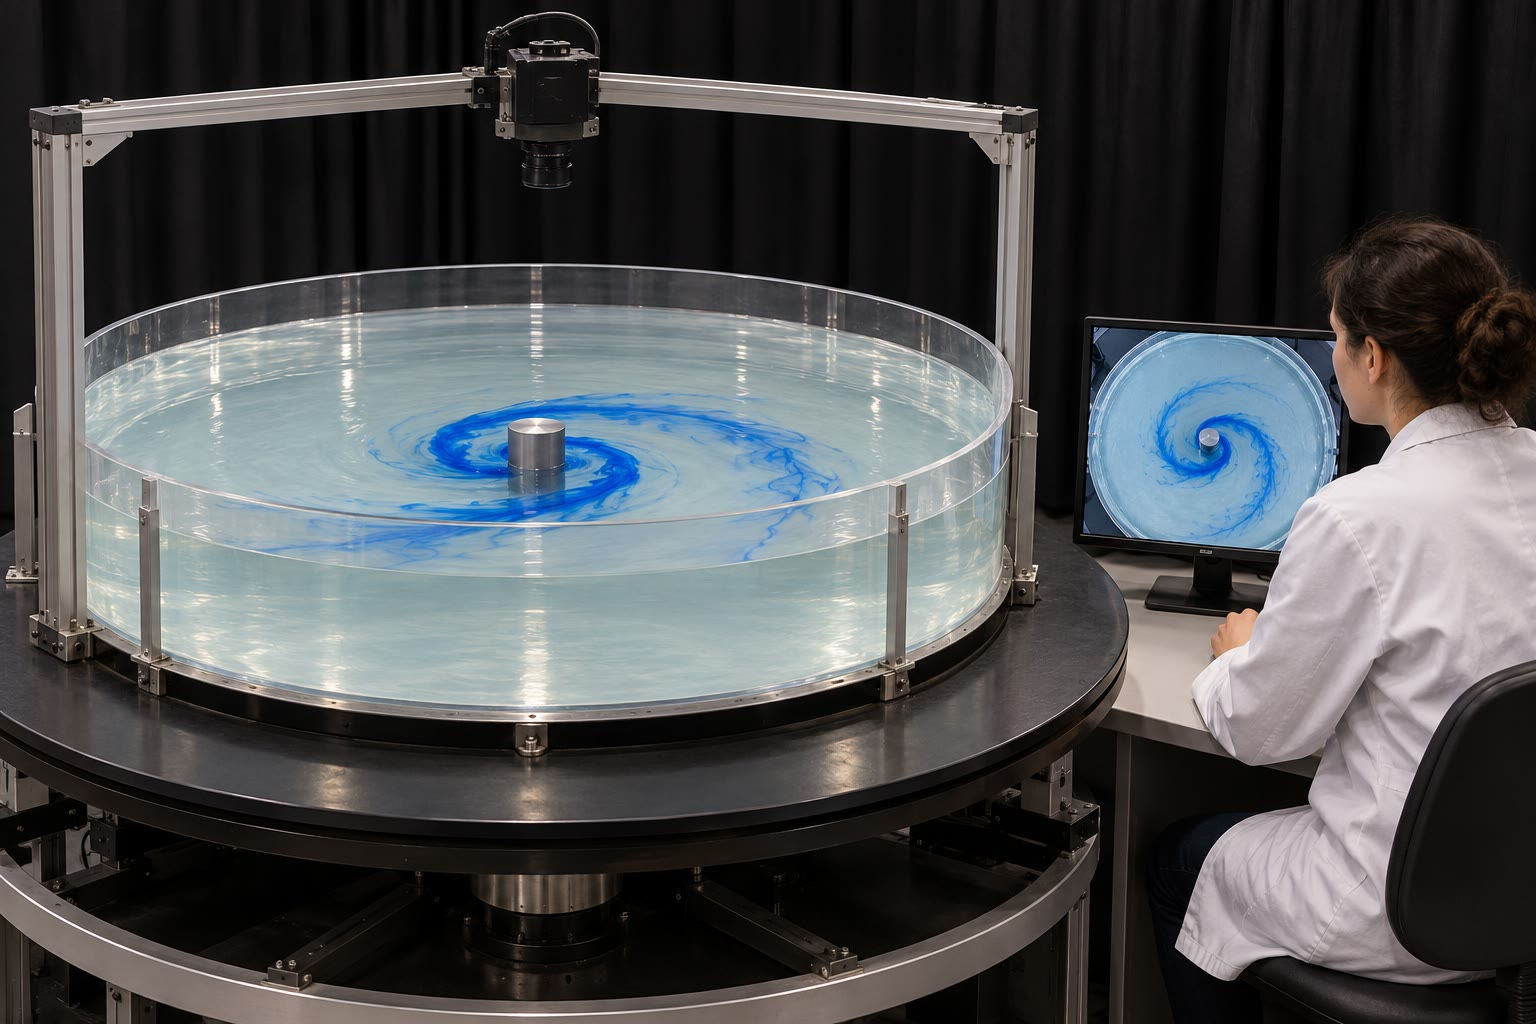
\includegraphics[width=\linewidth]{images/book5/ai/b3-rotating-tank.jpg}

{\scriptsize خزّان دوّار: صبغة تلتفّ حول أسطوانة، تصوّرها كاميرا
تدور مع الطاولة (رسم توضيحي مولَّد بالذكاء الاصطناعي).}
\end{minipage}
\end{inthelab}

\section{التمارين}

\begin{exercise}[$\star$]\label{exo:b3:gfd-foundations:1}
خذ $\Omega = \qty{7.292115e-5}{rad/s}$. (أ)~احسب معامل كوريوليس
والدور القصوري عند \ang{30}، \ang{45} و\ang{60} شمالًا.
(ب)~احسب نصف قطر الدائرة القصورية لتيار سرعته
\qty{0.20}{m/s} عند خطوط العرض نفسها. (ج)~قارن الدور القصوري عند
\ang{30} باليوم النجمي، \qty{23.9345}{h}.
\end{exercise}

\begin{exercise}[$\star$]\label{exo:b3:gfd-foundations:2}
عند \ang{45} شمالًا، احسب \omterm{def:b3:gfd-foundations:numbers}{عدد روسبي} لدوّامة غبارية (\qty{10}{m/s}،
\qty{10}{m})، ونسيم بحري (\qty{5}{m/s}، \qty{20}{km})، ومنخفض
جوي (\qty{15}{m/s}، \qty{1000}{km})، ودوّامة محيطية (\qty{0.05}{m/s}،
\qty{2000}{km}). أيّها قريب من التوازن الجيوستروفي؟
\end{exercise}

\begin{exercise}[$\star$]\label{exo:b3:gfd-foundations:3}
عند \ang{45} شمالًا يتناقص متوسط درجة الحرارة في التروبوسفير، \qty{250}{K}،
نحو الشمال بمقدار \qty{5}{K} لكل \qty{1000}{km}. باستخدام الحد الأول من
\omterm{thm:b3:gfd-foundations:thermal-wind}{الريح الحرارية} بدلالة الارتفاع، احسب القصّ الرأسي للريح الغربية،
ومقدار الزيادة في الريح عبر \qty{10}{km}.
\end{exercise}

\begin{exercise}[$\star$]\label{exo:b3:gfd-foundations:4}
يتراوح الاستقرار $E = -(1/\rho)\,\mathrm d\rho_\theta/\mathrm dz$ للكيلومتر العلوي من
المحيط بين \num{50e-8} و\qty{1000e-8}{m^{-1}}؛
وفي الخنادق العميقة يساوي \qty{e-8}{m^{-1}}. احسب $N = \sqrt{gE}$،
ودور تذبذب الطفو، و$N$ بوحدة دورات في الساعة لهذه
القيم الثلاث.
\end{exercise}

\begin{exercise}[$\star\star$]\label{exo:b3:gfd-foundations:5}
لدينا نظام طقسي $U = \qty{10}{m/s}$، $L = \qty{1000}{km}$، $H =
\qty{10}{km}$، عند \ang{45} شمالًا. (أ)~قدّر سرعته الرأسية وتسارعه الرأسي،
وقارن هذا التسارع مع $g$ ومع
التدرّج الرأسي لاضطراب الضغط، $fUL/H$. (ب)~احسب
حدّ كوريوليس المُهمَل $\tilde fu$ وقارنه مع $g$.
\end{exercise}

\begin{exercise}[$\star\star$]\label{exo:b3:gfd-foundations:6}
خذ $f = \qty{e-4}{s^{-1}}$ وخطوط تساوي الضغط الدائرية ذات نصف القطر
\qty{300}{km}. (أ)~يعطي تدرّج الضغط حول منخفض $V_g =
\qty{20}{m/s}$: احسب \omterm{def:b3:gfd-foundations:gradient}{الريح التدرّجية}. (ب)~حول مرتفع،
$V_g = \qty{5}{m/s}$: احسب \omterm{def:b3:gfd-foundations:gradient}{الريح التدرّجية}. (ج)~ما أكبر
$V_g$ ممكنة حول المرتفع، وما الريح عندئذٍ؟
\end{exercise}

\begin{exercise}[$\star\star$]\label{exo:b3:gfd-foundations:7}
يدور خزّان عمقه \qty{20}{cm} دورة كاملة كلّ \qty{6}{s}؛ ويبلغ لزوجة مائه $\nu =
\qty{e-6}{m^2/s}$. (أ)~احسب $f = 2\Omega$، ثم \omterm{def:b3:gfd-foundations:numbers}{عدد روسبي} لتدفّق
بسرعة \qty{1}{cm/s} حول أسطوانة قطرها \qty{5}{cm}، \omterm{def:b3:gfd-foundations:numbers}{وعدد إيكمان}
للخزّان. هل سيتشكّل \omterm{thm:b3:gfd-foundations:taylor-proudman}{عمود تايلور}؟ (ب)~تُعطي النظرية زمن طور التهيئة
$H/\sqrt{\nu\Omega}$: احسب الزمن بالدقائق وبعدد دورات الطاولة.
\end{exercise}

\begin{exercise}[$\star\star$]\label{exo:b3:gfd-foundations:8}
في المتوسط النطاقي لشهر يناير للفترة 1991--2020 تبلغ الريح الغربية \qty{4.27}{m/s}
عند \qty{850}{hPa} و\qty{40.39}{m/s} عند \qty{250}{hPa}، عند \ang{30} شمالًا،
\qty{5.99}{m/s} و\qty{23.17}{m/s} عند \ang{45} شمالًا. مع $R =
\qty{286.9}{J.kg^{-1}.K^{-1}}$، احسب التدرّج الزوالي لمتوسط درجة حرارة
الطبقة عند خطّي العرض كليهما، وبيّن لماذا يكون التيّار النفّاث أقوى
عند \ang{30} شمالًا.
\end{exercise}

\begin{exercise}[$\star\star$]\label{exo:b3:gfd-foundations:9}
(أ)~احسب \omterm{def:b3:gfd-foundations:rossby-radius}{نصف قطر روسبي للتشوّه} في التروبوسفير ($N =
\qty{0.0113}{s^{-1}}$، $H = \qty{11}{km}$، \ang{45} شمالًا) وفي المحيط العلوي
($N = \qty{0.00357}{s^{-1}}$، $H = \qty{1000}{m}$، \ang{40.5} شمالًا).
(ب)~مع $a = \qty{6371}{km}$، احسب $\beta$ عند خطّي العرض كليهما، والتغيّر النسبي
$\beta L_R/f$ لمعامل كوريوليس عبر كلّ نصف قطر.
\end{exercise}

\begin{exercise}[$\star\star\star$]\label{exo:b3:gfd-foundations:10}
تتباطأ كتلة من ماء السطح تتحرّك بالسرعة $U$ بفعل احتكاك
خطّي: $\mathrm du/\mathrm dt = fv - ru$، $\mathrm dv/\mathrm dt = -fu -
rv$. (أ)~حُلّ باستعمال $w = u + \mathrm iv$ وصِف المسار. (ب)~يُحمل
الجسيم أيضًا بتيار ثابت $u_0$ متجهًا شرقًا: أعطِ موضعه.
(ج)~عند \ang{45} شمالًا، مع $U = \qty{0.2}{m/s}$، $r^{-1} =
\num{4}\text{ يومًا}$ و$u_0 = \qty{0.05}{m/s}$، أعطِ سرعته بالنسبة إلى
التيّار بعد أربعة أيام، والمسافة التي انجرفها.
\end{exercise}

\begin{exercise}[$\star\star\star$]\label{exo:b3:gfd-foundations:11}
عبر جبهة محيطية عند \ang{40}~شمالًا تزداد كثافة الماء
نحو الشمال بمقدار \qty{1}{kg/m^3} على مسافة \qty{100}{km}، عبر الطبقة العليا
\qty{1000}{m}؛ وتحتها يكون الماء متجانسًا وساكنًا. مع $\rho_0 =
\qty{1025}{kg/m^3}$، احسب القصّ الرأسي للتيّار،
والتيّار عند السطح. في أيّ اتجاه يجري؟
\end{exercise}

\begin{exercise}[$\star\star\star$]\label{exo:b3:gfd-foundations:12}
العمود المتوسط السنوي عند \ang{40.5}~شمالًا، \ang{30.5}~غربًا له كثافات كامنة
$\sigma_\theta = \rho_\theta - \qty{1000}{kg/m^3}$ تبلغ 26.029 عند
السطح، 26.697 عند \qty{100}{m}، 27.079 عند \qty{500}{m}، و27.628 عند
\qty{1000}{m}. (أ)~احسب $N$ في كلّ طبقة من الطبقات الثلاث، بوحدة
\unit{s^{-1}} وبالدورات في الساعة. (ب)~أيّ الطبقات هي الأكثر استقرارًا،
ولماذا؟ (ج)~قارن القيم بمدى المحيط العلوي في
\cref{exo:b3:gfd-foundations:4}.
\end{exercise}
% ledger: geod5:grs80-defining, earth:Trot, stewart:stability, data:b5-ncep-uwnd, data:b5-woa23-atlantic, earth:Rmean

\section{مسألة: الرياح فوق سهوب أورين}

\begin{problem}[{مسألة نهاية الأسبوع --- الدوران والتطبّق والرياح
في سهل مُخترع عند \ang{48}~شمالًا}]
\label{pb:b3:gfd-foundations:1}
سهوب أورين سهلٌ مستوٍ عند \ang{48}~شمالًا، فيه بحيرة، هي بحيرة أورين،
عرضها \qty{12}{km}، ومختبرٌ صغير فيه خزّان دوّار. خذ
$\Omega = \qty{7.292115e-5}{rad/s}$, $g = \qty{9.81}{m/s^2}$, $R =
\qty{286.9}{J.kg^{-1}.K^{-1}}$ و$c_p = \qty{1004}{J.kg^{-1}.K^{-1}}$.
جميع قيم السهوب وبحيرتها ورياحها مُخترعةٌ.

\medskip\noindent\textbf{الجزء الأول --- هل للدوران أهمية؟}
\begin{enumerate}
\item احسب معامل كوريوليس ودور \omterm{def:b3:gfd-foundations:inertial}{الاهتزاز القصوري} عند أورين.
\item احسب \omterm{def:b3:gfd-foundations:numbers}{عدد روسبي} لخمسة تدفّقات: مياه تنصرف من حوض الاستحمام
  (\qty{0.1}{m/s} على مسافة \qty{0.3}{m})؛ خزّان المختبر، الذي يدور
  مرّةً كلّ \qty{10}{s} (مع $f = 2\Omega_{\text{الخزّان}}$؛ \qty{5}{mm/s}
  على مسافة \qty{0.2}{m})؛ نسيم المساء القادم من البحيرة (\qty{5}{m/s}،
  \qty{20}{km})؛ منخفض جوي (\qty{15}{m/s}، \qty{1000}{km})؛ الدوّامة المحيطية لحوضٍ
  محيطي عند خط العرض نفسه (\qty{0.05}{m/s}، \qty{2000}{km}).
\item أيّ هذه التدفّقات يشعر بالدوران الذي يحرّكها، وأيّ منها
  قريب من الجيوستروفي؟
\item احسب \omterm{def:b3:gfd-foundations:numbers}{عدد إيكمان} للخزّان (عمقه \qty{0.2}{m}، $\nu =
  \qty{e-6}{m^2/s}$)، وللمنخفض (اللزوجة الدوّامية \qty{10}{m^2/s}،
  عمقه \qty{10}{km})، وللدوّامة المحيطية (اللزوجة الدوّامية \qty{e-3}{m^2/s}،
  عمقها \qty{1000}{m}).
\item لطبقة إيكمان سُمك $\delta = \sqrt{2\nu/f}$. بيّن أنّ
  $\delta/H = \sqrt{2\,\mathrm{Ek}}$ واحسب $\delta$ للخزّان وللهواء
  في السهوب.
\item ماذا تقول هذه الأعداد عن المواضع التي يكون فيها للاحتكاك أهمية؟
\end{enumerate}

\medskip\noindent\textbf{الجزء الثاني --- الريح عند سطح الأرض.}
\begin{enumerate}[resume]
\item عند سطح الأرض يكون الضغط \qty{1012.9}{hPa} ودرجة الحرارة
  \qty{288.1}{K}. احسب كثافة الهواء.
\item ينخفض ضغط مستوى سطح البحر نحو الشمال بمقدار \qty{4}{hPa} لكلّ
  \qty{300}{km}. احسب الريح الجيوستروفية وأعطِ اتجاهها.
\item التدرّج نفسه يحيط بمنخفض تبلغ أنصاف أقطار خطوط تساوي ضغطه
  \qty{600}{km}. احسب \omterm{def:b3:gfd-foundations:numbers}{عدد روسبي} لخطوط تساوي الضغط \omterm{def:b3:gfd-foundations:gradient}{والريح
  التدرّجية}.
\item يحيط بالمرتفع الجوي التدرّجُ نفسه وبنصف القطر نفسه.
  احسب \omterm{def:b3:gfd-foundations:gradient}{الريح التدرّجية}، وأكبر تدرّج للضغط، بوحدة
  \unit{hPa} لكلّ \qty{300}{km}، الذي يستطيع المرتفع الجوي حمله.
\end{enumerate}

\medskip\noindent\textbf{الجزء الثالث --- التطبّق.}
\begin{enumerate}[resume]
\item تنخفض درجة حرارة التروبوسفير بمقدار \qty{6.49}{K/km}.
  احسب معدّل التناقص الأديباتي الجاف $g/c_p$، و$N$ ودور
  اهتزاز الطفو عند \qty{5}{km}، حيث تبلغ درجة الحرارة
  \qty{255.7}{K}.
\item فوق \qty{11}{km} يكون الهواء متساوي الحرارة عند \qty{216.6}{K}. بيّن أنّ
  $N^2 = g^2/(c_pT)$ هناك، واحسب $N$ ونسبته إلى
  قيمة السؤال~11.
\item احسب نصف قطر روسبي لتروبوسفير أورين، مستخدمًا $N$ من
  السؤال~11 و$H = \qty{10}{km}$، وقارنه بحجم المنخفض في
  الجزء~I.
\item في الصيف، تكون الطبقة العليا من بحيرة أورين، بسُمك \qty{20}{m}، أخفّ من
  الماء العميق بمقدار \qty{1.5}{kg/m^3} ($\rho_0 = \qty{1000}{kg/m^3}$). احسب
  الجاذبية المختزلة $g' = g\,\Delta\rho/\rho_0$، وسرعة $\sqrt{g'h}$ للأمواج
  الداخلية البطيئة في الطبقة العليا، ونصف قطر روسبي
  $\sqrt{g'h}/f$.
\item هل سيشكّل دوران الأرض الحركات الداخلية في البحيرة؟
\end{enumerate}

\medskip\noindent\textbf{الجزء الرابع --- \omterm{thm:b3:gfd-foundations:thermal-wind}{الريح الحرارية}.}
\begin{enumerate}[resume]
\item تبعد محطّتان للمسبار الراديوي \qty{600}{km} إحداهما عن الأخرى على
  خطّ الزوال نفسه. متوسط درجة الحرارة للطبقة من سطح الأرض،
  \qty{1013}{hPa}، حتى \qty{265}{hPa}، نحو \qty{10}{km}، يبلغ \qty{253.0}{K}
  عند المحطّة الجنوبية، و\qty{249.4}{K} عند المحطّة الشمالية. احسب
  التدرّج الحراري الزوالي بوحدة \unit{K} لكلّ \qty{1000}{km}.
\item سُمك الطبقة المحصورة بين ضغطين هو $\Delta z = (R\bar
  T/g)\ln(p_b/p_t)$. احسب هذا السُّمك عند المحطّتين، وميل سطح
  \qty{265}{hPa} بالنسبة إلى السطح عند مستوى الأرض.
\item استنتج الزيادة في الريح الجيوستروفية من سطح الأرض حتى
  \qty{265}{hPa}، من هذا الميل.
\item احسب الزيادة نفسها بمبرهنة \omterm{thm:b3:gfd-foundations:thermal-wind}{الريح الحرارية} في الضغط.
\item هل هواء السهوب \omterm{def:b3:gfd-foundations:baroclinic}{باروتروبي} أم \omterm{def:b3:gfd-foundations:baroclinic}{باروكليني}؟ ما الريح عند
  \qty{265}{hPa} لو كان الهواء باروتروبيًّا؟
\item احسب الزيادة من الحدّ الأول للريح الحرارية في
  الارتفاع، مع متوسط درجة الحرارة للتروبوسفير المعياري بين 0
  و\qty{10}{km}، \qty{255.7}{K}، وقارِن.
\item احسب الريح عند \qty{541}{hPa}، نحو \qty{5}{km}، مفترضًا أنّ
  التدرّج الحراري هو نفسه عند كلّ مستوى.
\item يجب أن ينخفض عدد ريتشاردسون $N^2/(\partial u/\partial z)^2$ إلى ما دون
  0.25 حتى يولّد القصّ اضطرابًا. احسب هذا العدد للتروبوسفير في
  أورين.
\item في يناير يبلغ المتوسط النطاقي للريح الغربية عند \qty{250}{hPa}
  \qty{23.2}{m/s} عند \ang{45}~شمالًا و\qty{40.4}{m/s} عند \ang{30}~شمالًا. قارِن بالريح في
  أورين، واشرح لماذا يمكن للريح المحلّية أن تتجاوز المتوسط النطاقي.
\item أعطِ الريح الجيوستروفية عند \qty{10}{km} فوق سهوب أورين.
\end{enumerate}
\end{problem}
% ledger: geod5:grs80-defining, stewart:stability, data:b5-ncep-uwnd, nasa:grc-atmos
